% !TEX encoding = UTF-8
% !TEX TS-program = pdflatex
% !TEX root = ../tesi.tex

%**************************************************************
\chapter{Deep learning}
\label{cap:deep-learning}
%**************************************************************

\intro{In this chapter I will dive deep (no pun intended) in the reasons behind the choice of a deep learning approach to detect custom-class objects in image data.}\\

%**************************************************************
\section{Overview}
	\emph{Deep learning} is a part of the broader family of \emph{\gls{machine learning}}\glsfirstoccur methods that focuses on learning features of interest by experiencing them thought data samples. In contrast to \emph{machine learning}, which still needs the problem's layout to be described by a rather complex human-coded algorithm, a \emph{deep learning} model only needs a dataset to autonomously learn from. Thanks to the ever-growing availability of computational power and labeled data, and the relative simplicity in which a network can be trained, the deep learning approach to solve artificial intelligence problems is flourishing, bringing artificial intelligence to everyday life. \\
	At the core of every \emph{deep learning} model there is an artificial neural network, whose architecture is strongly inspired by the structure and functioning of a biological brain. Basically, an artificial neural network is composed by a variable number of neuron layers densely connected and stacked upon each other, hence the name \emph{deep neural networks}. The information is elaborated by traveling from layer to layer until the top is reached. \\
		As stated, each layer is composed of computational units that work like \emph{neurons}: each \emph{neuron} receives an input, and using an activation function it produces an output that propagates to activate a \emph{neuron} in the following layer. Actually each \emph{neuron}'s output is influenced by weights and thresholds that need to be adjust to achieve the best performance.
	 When learning, the network indeed adjusts the weights and thresholds that activate each \emph{neuron}'s function, so that it can get closer to the wanted result in an iterative manner. After each passage through the network, a \emph{\gls{loss function}}\glsfirstoccur is calculated to determine how well it is performing; then a \emph{\gls{gradient descent function}}\glsfirstoccur derives how this performance can be improved by decreasing the loss and accordingly \emph{\gls{back-propagation}}\glsfirstoccur is performed to adjusts the weights used by the neurons in their activation functions.
	 
\begin{figure}[htbp]
\begin{center}
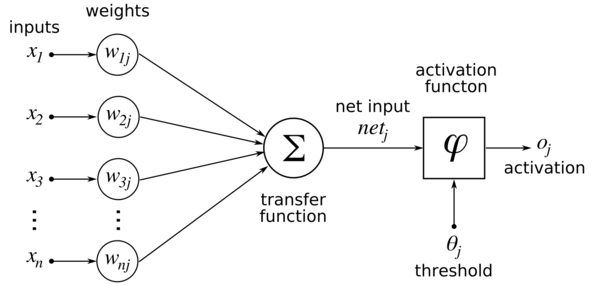
\includegraphics[width=\textwidth]{immagini/pictures/neuron.png} 
\caption{Visual representation of the activation function that determines a neuron's output and the parameters that influence it.}
\end{center}
\end{figure}	

\begin{figure}[htbp]
\begin{center}
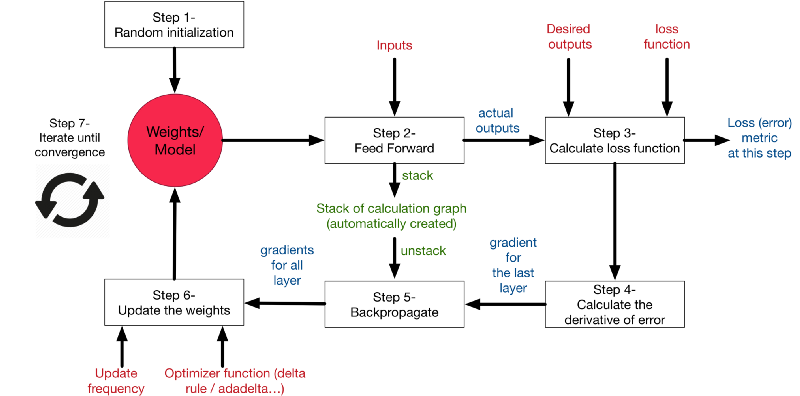
\includegraphics[width=\textwidth]{immagini/pictures/training.png} 
\caption{Schematic representation of how a network updates the weight to decrease the loss and achieve better accuracy.}
\end{center}
\end{figure}
	
\section{Deep neural networks}
	As mentioned above, the \emph{deep learning} approach to solve a problem is to train a \emph{deep neural network} to recognize the wanted features so it can later make predictions about them. Basically when you train a \emph{deep neural network} you feed it thousands of data samples, so it can learn from the wanted data representation by "seeing" it, just like you would show a child pictures of kittens to teach him what a kitten is.
	There are two different ways to train a network, each one with different goals and contexts of use:
	\begin{itemize}
		\item supervised training: the network is given a labeled \emph{\gls{dataset}}\glsfirstoccur to learn from; for each data sample the ground truth is provided, so the network knows what it is learning. This is the preferred approach whenever labeled data is available.
		\item unsupervised training: the network is given an unlabeled \emph{dataset} to learn from; no ground truth is given, so the network has to identify patterns and divide them into different categories on its own. This approach is preferred when the goal is to group data in categories or when data is too complex to be labeled.
	\end{itemize}
	There are different network architectures, each one dedicated to a specific type of problems. When solving  \emph{\gls{computer vision}}\glsfirstoccur task the best performances are held by a class of networks called \emph{convolutional neural networks}. \\

	\subsection{Convolutional neural networks}
	\emph{convolutional neural networks} (CNNs) are \emph{deep neural networks} that consist of an input layer, an output layer, and a variable number of hidden layers with different purposes. What names this family of networks is in fact on particular type of layer, called \emph{convolutional layer}; a single network typically contains various \emph{convolutional layers} of different size, and each perform a \emph{convolution} operation that filters its input stimuli before passing them the to next layer in order to reduce the parameters number, thus allowing the network to be deeper. \\
	CNNs, among others, are mainly used to perform computer vision tasks; in particular they achieve good results in object detection tasks. \\

\begin{figure}[htbp]
\begin{center}
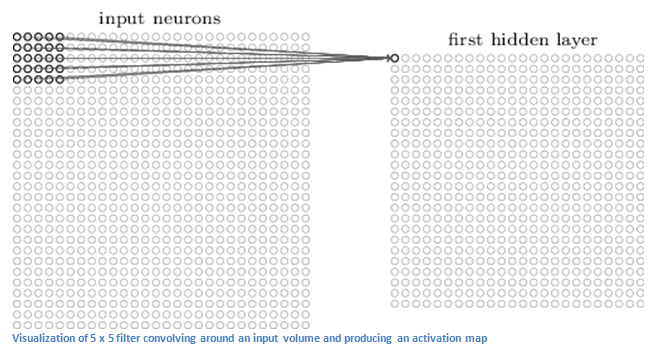
\includegraphics[width=\textwidth]{immagini/pictures/ActivationMap.png} 
\caption{Visual representation of a convolutional layer.}
\end{center}
\end{figure}

	\subsection{Object detection}
	\emph{Object detection} is a computer vision problem that concerns the identification of class instance objects in an image (or video), and locating the actual position of said object in the picture. Commonly the spacial orientation of the detected object is framed by a rectangular \emph{bounding box} that determines its height and width. Thus, object detection is far more powerful than mere image classification, not only because it "draws" a box where the object is located, but also because it can identify multiple object instances in a single image, while classification models have the limit of labeling only the one predominant object in the scene. The capability of labeling and locating multiple instances opens object detection models to a new set of application, such as video surveillance (e.g. moving subjects can be tracked) and instance counting for industrial purposes (e.g. counting boxes in a warehouse). Furthermore, object detection has proven to be more reliable than classification to scan images where the subject of interests occupies only a small part of the picture (e.g. a street sign in the corner). \\
	Commonly an \emph{object detection} model is actually built on top a classifier that works as a \emph{feature extractor}, but this exudes the topics of my project and I am introducing this notion only because it is noticeable in the naming convention of model networks, which are indeed important in my work. \\
	There are three popular network architectures for object detection:
	\begin{itemize}
		\item SSD (Single Shot Detection);
		\item R-CNN (Region-based \emph{convolutional neural network}, and its upgrades Fast R-CNN and Faster R-CNN);
		\item YOLO (You Only Look Once).
	\end{itemize}
While both \emph{SSD} and \emph{YOLO} follow the same approach of computing the image data through a single network, \emph{R-CNN} splits the image in various regions trying to guess where objects of interest might be and processes each area separately, thus requiring more computational power. State-of-the-art models share comparable performances in accuracy, but due to the time overhead of processing a picture multiple times, \emph{R-CNN} is a bit slower than \emph{SSD} and \emph{YOLO}.

\begin{figure}[htbp]
\begin{center}
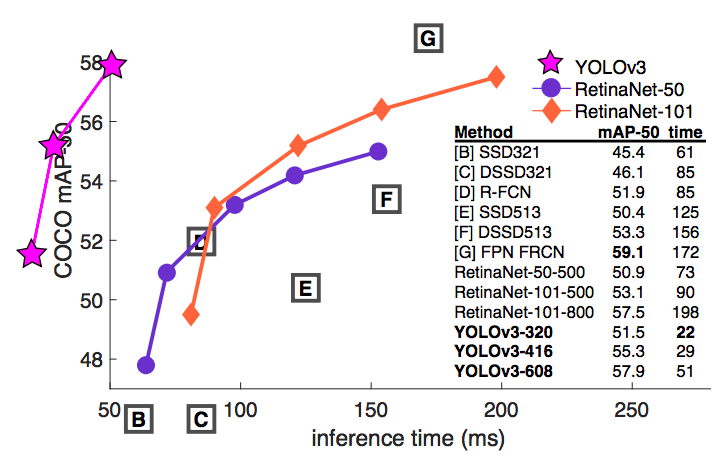
\includegraphics[width=\textwidth]{immagini/pictures/netcomparison.png} 
\caption{Comparison on object detection performances on Nvidia Titan X GPU. A higher mAP value means a better accuracy.}
\end{center}
\end{figure}

\subsection{YOLO v3}
	\emph{YOLO}\footnote{\url{https://pjreddie.com/darknet/yolo/}} is a \emph{convolutional neural network} built on top of \emph{Darknet} classifier, now on its third version \emph{YOLO v3}. Both \emph{YOLO} and \emph{Darknet} are developed by Joseph Redmon on his C-written open source neural network framework Darknet\footnote{To avoid misunderstandings I will call Darknet the framework and \emph{Darknet} the classifier.}. \\
	What makes \emph{YOLO} stand out compared to its competitor is its speed: at par of accuracy YOLO can perform inference in less than half the time, achieving the ability to track moving subjects in real time in 30fps videos using a gaming-tier GPU\footnote{Real time inference is possible on Nvdia GeForce Titan X GPU.}. \\
	For my project I was asked to used \emph{YOLO} in its newest version, \emph{YOLO v3}. As I already said, \emph{YOLO} was firstly implemented in Joseph Redmon's Darknet framework, which is written in C so it is fast, but unfortunately it is suitable only for research purposes. Since I was asked to develop a production-ready application, I had to choose another framework to work on, and I will discuss about it in later chapters.
	
	\subsubsection{Structure}
	\emph{YOLO v3} is an \emph{convolutional neural network} for \emph{object detection} built on top of \emph{Darknet53}, an image classifier that uses 53 convolutional layers. With \emph{Darknet53} as its feature extractor, \emph{YOLO}  processes every image once, looking at it as a whole, hence encoding extra information about the context each class lives in. To do so it models detection as a regression
problem, dividing the image into an S $\times$ S grid, and for each grid cell predicts B bounding boxes, confidence for those boxes, and C class probabilities; when a class-object's center falls inside a grid cell, that grid cell is responsible of detecting that object.
	
	\begin{figure}[htbp]
\begin{center}
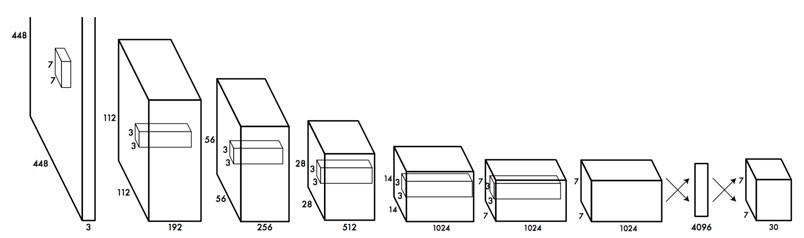
\includegraphics[width=\textwidth]{immagini/pictures/yololayers.jpeg} 
\caption{Visual representation of \emph{YOLO} network layers in its first version.}
\end{center}
\end{figure}

	
\section{Training a network}
	Training a \emph{convolutional neural network} is a computation-heavy task, that involves the processing of thousands of pieces of data, which in the context of computer vision is in the format of images. Therefore best way to process thousands of images is to use a GPU; using a GPU (or even clusters of GPUs) it is possible to process the images in parallel among the \emph{cores}, speeding up the process greatly. As a comparison, while training on CPU would take days even on a small dataset, on a GPU all the work would be done in just few hours.
	\subsection{Dataset}
	The first and most important step to train a network is to create the \emph{dataset} it will learn from. Note that the quality of the dataset itself will have great influence on the final accuracy of the network. For instance you will want to feed your network examples of your objects of interest from every perspective and immerse in their context; also, when training a network to perform an \emph{object detection} task, you want your \emph{bounding boxes} to be as accurate and tight around the figures as possible. \\
	Clearly, creating a custom dataset is a demanding job, since piece of data must be manually labeled by a human. For my project I was given a custom dataset created by one of my colleagues, containing classes relevant for one of THRON's clients. Creating a \emph{dataset} exudes the goals of my project, since on production it will be possibly performed by clients\footnote{As explained in the introduction, THRON's product is a DAM, which in this context can basically seen as a database of categorized images; with possibly minor changes to data labeling (e.g. introduction of bounding boxes for the objects of interest) and database export, image data can be easily turned into a dataset for computer vision.}. \\
	When creating an \emph{object detection} \emph{dataset} there are there are two main qualities to determine its goodness:
	\begin{itemize}
		\item \emph{Cardinality}, which is the means of the number of labels per image;
		\item \emph{Density}, which is the cardinality divided by the number of classes.
	\end{itemize}
A density too low has negative influence on the final accuracy of the network, because basically you are trying to teach it to recognize a high number of classes, but you're giving it only a few examples for each. On a lesser degree, a cardinality too high has  a negative influence on the final accuracy as well because the examples you are giving are too cluttered with information. Furthermore, when creating your own \emph{dataset}, you might want to insert a similar amount image samples/labels for each class. \\
After the full dataset is created, it is common practice to divide it into two separate \emph{datasets}: a \emph{training dataset} and a \emph{validation dataset}, with the suggested ratio of 70\% training and 30\% validation. Note that these two \emph{datasets} contain different samples to avoid \emph{\gls{overfitting}}\glsfirstoccur.

	\subsection{Training}
	Once the dataset is ready and formatted in the network's preferred format\footnote{Depending on the framework, the preferred format changes. To work with YOLO v3 on MXNet data can provided in both RecordIO format or LST + Jpeg format.}, the training process can begin. \\
	The training process is conceptually simple; as previously stated, teaching a machine to recognize kittens can be compared to showing pictures to a child and pointing at the kitten in them to make him understand what a kitten is. When doing so with a child you only need a few examples, when with a machine you'll probably need a few hundreds. The next step is to check whether the machine truly learned what a kitten is; again this can be roughly compared to checking whether the child truly learned what a kitten is by giving him a picture and asking him to point at the kitten, if there is one. \\
	Now that we talked about kittens and children we can explore in detail how a machine learns the way a human would.
	The training process is a loop in which the network is "shown" the \emph{dataset} it should learn from; since a \emph{dataset} is composed by thousands of images, it can't be entirely loaded into memory and must be split in smaller units for processing, called \emph{batches}; in practice maximum \emph{batch} size is determined by your hardware specifics. Your network will be fed all of the training \emph{dataset} \emph{batch} after \emph{batch}. Each loop of computation on the whole training dataset is called an \emph{\gls{epoch}}\glsfirstoccur. To train your network you will want to perform at least a couple of hundreds epochs; this means that to learn the \emph{dataset} your network will go through all of it hundreds of times. 

	\subsection{Validation}	
	Every fixed epoch number you will want to check your network's learning progress; to do so you will perform a validation loop, which means that you will feed the network your validation \emph{dataset} and compare the network's prediction with the ground truth. There are various metrics to calculate a network's accuracy, and the one I used on my project is called \emph{\gls{mean average precision}}\glsfirstoccur (mAP). This evaluation metric uses an \emph{\gls{intersection over union}}\glsfirstoccur (IoU) threshold to determine how well the detected positives overlap with the ground truth; setting the IoU threshold higher or lower influences the wanted precision at locating objects\footnote{Note that ground truth bounding boxes are hand-drawn by a human so they already come with an error, thus setting the IoU threshold too high could prove to be useless and even counterproductive.}, and I set it to a value of 0.5.
	
	\subsection{Transfer learning}
	Training a network from scratch is a quite demanding operation in terms of computational time and power, because the weights for each class need to be calculated from a random initialization. Luckily, it is possible to train a network to recognize new custom classes starting from pre-trained weights for other (general) classes, and this process is called \emph{transfer learning}. \\
	 Basically when you apply transfer learning on a pre-trained network\footnote{All the major deep learning frameworks usually provide networks and weights pre-trained on popular datasets such as COCO, Pascal VOC or ImageNet.}, you teach it to recognize new classes by adjusting its weights (which have a meaning and are not random anymore) and the structure of the two layers that determine the final output. To benefit from \emph{transfer learning}
	 you want to choose a base network with weights for classes that share some features with your custom ones for example if you want to be able to detect different species of animals, a good choice would be to \emph{fine-tune} a network trained on a datasets that already contains cats and dogs.
	
	\subsection{Hyperparameters}
	The accuracy of a \emph{convolutional neural network} is influenced by various paramenters, called hyperparameters, that tweak how the weights are updated and how the results are evaluated. This values come in the form of \emph{"magic numbers"}, meaning that for every dataset each network has its own values to optimize the final performance and that they can be found only in a trial and error fashion\footnote{To determinate the best values it is common practice to re-train the network various times and compare the results.}. Since this is rather time consuming, especially when training on CPU, I couldn't tune the hyperparameters for my project. However I will introduce briefly what the main hyperparameters do on a \emph{YOLO v3} architecture network.
	\begin{itemize}
	\item Learning rate. Speed at which the network learns. It is used when updating weights and a learning rate too high might cause overfitting.
	\item Learning rate deacay rate. As the network learns, its learning rate decreases; this value is important to avoid overfitting.
	\item Momentum. Stochastic gradient descent momentum, used by the gradient descent function to calculate how to reduce the loss.
	\end{itemize}

\section{Object detection for THRON}
	As mentioned in Chapter 1, THRON already uses generic classification services in its \emph{DAM}. Therefore, to provide a better service, it comes natural that the Company has interest in developing a system able to detect custom classes. \\
	Since THRON already has a vast database of labeled data, following a deep learning approach is the easiest option, even more so now that framework providing almost out-of-the-box are increasing prominence. \\
	At first it was still unclear whether the Company needed just a classifier, but with my proof-of-concept the benefits of an \emph{object detection} model became clear. We particularly chose \emph{YOLO v3} under the suggestion of a data scientist working in my team, since he already developed a research-purpose prototype application using \emph{YOLO v2}. Due to the technology used, his application couldn't be released in a production environment, so it was my job to develop a production-ready application using \emph{YOLO}.